\subsection{PageRank vs Orden Total Conocido}
\label{subsec:exp5}
\begin{LaTeXdescription}
    \item[Objetivo] Analizar la convergencia del modelo GeM asumiendo que
        existe ranking ideal y correcto al cual converger.\\

    \item[Hip\'otesis] PageRank, utilizando el modelo GeM, converge finalmente a
        un ''Orden Real'' o ''Correcto'' de los competidores, si este existe.
        Adem\'as, no necesitar\'a de un grafo completo (los resultados de todos
        contra todos) para converger al mismo.\\

    \item[Proposici\'on] Como se coment\'o previamente en la experimentaci\'on
        sobre p\'aginas web, establecer cual es el ''mejor orden'' u ''orden
        correcto'' es completamente arbitrario. No hay una vara sobre la cual
        medir. En los deportes esto es a\'un más evidente, ya que se depende de
        los resultados deportivos, ¿y qui\'en es capaz de afirmar que la
        probabilidad de que Platense -el mejor equipo del mundo e insipirador
        del t\'itulo del enunciado de este trabajo- le gane al Barcelona es $0$?
        As\'i pues, en el caso de los deportes tampoco tenemos un orden total,
        conocido y determin\'istico para verificar que el resultado de PageRank
        es el correcto. Pero si existiese este orden, si fuese determin\'istico,
        ¿PageRank convergir\'ia al mismo?\\

    \item[M\'etodo de Experimentaci\'on] Generamos dos instancias ideales y
        completamente abstractas de los resultados de un torneo de f\'utbol con
        10 y 50 equipos respectivamente, que juegan todos contra todos una
        \'unica vez (45 partidos para la primera instancia, 1225 para la
        segunda). Las instancias son construidas de manera tal que $equipo_i$ le
        gana a $equipo_j$ si y s\'olo si $i<j$. Es decir, el ranking correcto es
        la numeraci\'on de los equipos de forma ascendente, y cada $equipo_i$
        ocupa el puesto $i$.

        \par Aprovechamos el hecho de que en los deportes hay una componente
        temporal y generamos los partidos por fecha (es decir, grupos de
        partidos que ocurren todos al mismo tiempo, o al menos as\'i ser\'a para
        la perspectiva del algoritmo, que recibir\'a todos los partidos de una
        fecha juntos). En cada fecha se enfrentan, de a dos, equipos que no se
        hayan enfrentado todav\'ia y que no jueguen otro partido esa misma
        fecha. Dentro de esas restricciones, los enfrentamientos de cada fecha
        se eligen al azar, pero con una semilla fija (5) para obtener
        reproducibilidad en los experimentos. \textbf{Notar que la cantidad de
        fechas necesarias para que se jueguen todos los partidos no est\'a
        determinada \'unicamente por la cantidad de equipos sino que depende
        tambi\'en de como se elijan los enfrentamientos de cada fecha. Esto se
        debe a que confeccionar un generador de instancias aleatorias que
        respete las restricciones y genere un fixture de $n-1$ equipos es
        complejo y escapa a los objetivos de este trabajo. As\'i pues, nuestra
        instancia de 10 equipos \underline{consta de 11 fechas} y la instancia
        de 50 equipos \underline{consta de 53 fechas}}.

        \par El resultado de todos los partidos es siempre 1 a 0. No hace falta
        considerar empates dado que siempre hay un ganador. Luego, ejecutamos
        GeM tantas veces como fechas haya, pas\'andole en cada instancia una
        fecha m\'as. Es decir, en la ejecuci\'on 1 le pasamos los resultados de
        la fecha 1, en la 2 los resultados de la fecha 1 y 2, y as\'i
        sucesivamente. Para cada resultado de GeM, comparamos el ranking
        obtenido con el correcto, para alguna medida de distancia entre
        rankings, que definiremos m\'as adelante.

        \par Hace falta considerar un detalle importante, que es qu\'e
        decisi\'on tomar ante empates del ''puntaje'' asignado por GeM. Si
        desempat\'aramos por n\'umero de equipo de manera ascendente caer\'iamos
        en el molesto caso de que ya desde antes de empezar el torneo la salida
        de GeM coincidir\'ia con el orden ideal. Lo mismo vale para cualquier
        subconjunto de competidores empatados en un momento dado: su orden
        relativo coincidir\'ia con el ideal, aunque por casualidad y no por
        virtud del algoritmo. Resolvimos entonces ''romper'' el caso y que el
        desempate se realice de manera descendente, asegur\'andonos as\'i de no
        tomar como correctos resultados en donde hay muchos empates.

        \par Repetimos el experimento variando los valores de $\alpha$ en
        factores de $0.2$, para estudiar la convergencia en cada caso.  De
        confirmarse nuestra hip\'otesis la diferencia/distancia del ranking
        respecto del orden total ideal (que sabemos que existe por
        construcci\'on) deber\'ia llegar a ser 0, eventualmente ''antes'' de que
        se hayan jugado todas las fechas.\\

    \item[Resultados, an\'alisis y discusi\'on]
\end{LaTeXdescription}

\par En primer lugar, como hemos adelantado, debemos decidir como determinar la
''distancia'' entre dos rankings. Es decir, determinar alguna manera de comparar
dos rankings dados, y poder tener una magnitud de cuan parecidos son. Para ello
consideramos algunas opciones para dados dos rankings A y B, de entre las cuales
mencionamos:

\begin{enumerate}
        \item La sumatoria de la distancia, para cada competidor, entre su
            posici\'on en el ranking A y la posici\'on en el ranking
            B.\label{itm:distancia_rankings}
\end{enumerate}

\par Luego de evaluar estas opciones (y algunas m\'as no tan concisas),
decidimos trabajar de aqu\'i en m\'as con la distancia basada en la suma de las
distancias de todos los competidores (definici\'on de distancia n\'umero
\ref{itm:distancia_rankings}). Consideramos que dicha forma de tomar la
distancia entre dos rankings, de alguna manera nos est\'a se\~nalando cuantas
permutaciones de elementos/equipos contiguos hay entre un ranking y el otro,
cosa que no queda tan claro con las dem\'as opciones. Y esa forma de medir la
distancia es la que consideramos que se ajusta a lo que queremos observar del
dominio del problema: cu\'antos equipos est\'an ubicados distinto y cuan lejos.

\begin{figure}[H]
    \centering
    \subfloat[][Torneo de 10 equipos]{
        \label{subfig:exp5_10equipos}
        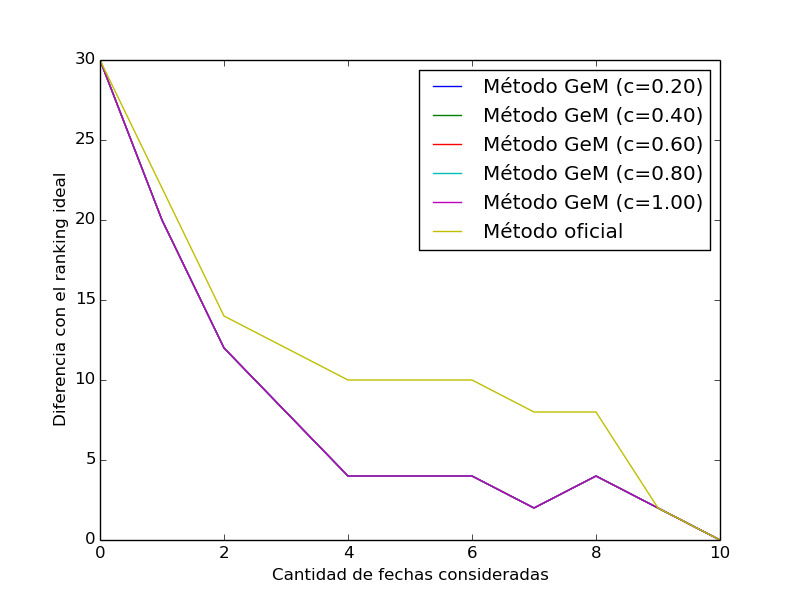
\includegraphics[width=.5\textwidth]{exp5_10_equipos.png}
    }
    \subfloat[][Torneo de 50 equipos]{
        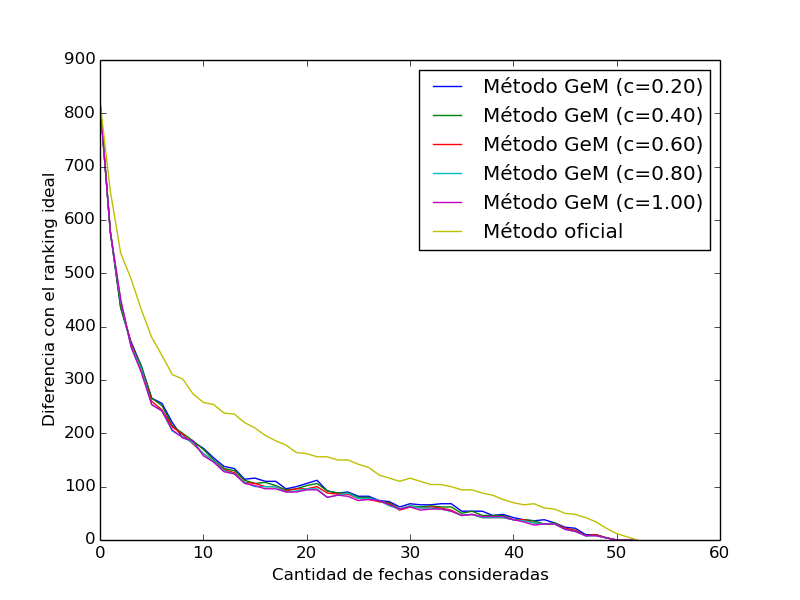
\includegraphics[width=.5\textwidth]{exp5_50_equipos.png}
        \label{subfig:exp5_50equipos}
    }
    \caption{Distancia al orden total ideal/correcto ($c = \alpha$)}
    \label{fig:exp5}
\end{figure}

\par La hip\'otesis fue confirmada. GeM converge al Orden Real para todos los
valores no nulos de $\alpha$ y no precisa todas las fechas para hacerlo, como se
puede observar en la figura \ref{fig:exp5}. Sin embargo, necesita una cantidad
significativa: para todos los valores no nulos de $\alpha$ fueron necesarias 10
de 11 fechas para el caso de 10 equipos y 50 de 53 fechas para el caso de 50
equipos.

\par El caso $\alpha=0$ no funciona porque la matriz termina descartando los
resultados de los equipos y usando simplemente la misma probabilidad para
cualquier equipo. En adelante dejaremos de lado este caso.

\par La variaci\'on $\alpha$ en el caso de 10 equipos no represent\'o
diferencias en el orden devuelto en cada fecha. es por eso que en la figura
\ref{subfig:exp5_10equipos} no se ven m\'as que dos curvas (una de las cuales
corresponde al siguiente experimento): estan todas superpuestas. En el caso de
50 equipos s\'i hubo leves diferencias en el orden devuelto en cada fecha.
Observamos que a mayor $\alpha$ el algoritmo en general converge ''mejor'' al
Orden Real (es decir, dada la misma cantidad de fechas, se acerca m\'as), aunque
siempre precisa 50 fechas para converger al orden real (figura
\ref{subfig:exp5_50equipos}).

\par La diferencia de todos modos es peque\~na y probablemente se deba a que, en
nuestro modelo ideal, las victorias son totalmente transitivas: la probabilidad
de que $C$ le gane a $A$ dado que $A$ le gan\'o a $B$ y $B$ le ganó a $C$ es
siempre $0$.  Como valores peque\~nos de $\alpha$ tienden a agregar una
probabilidad de que $C$ efectivamente le gane a $A$, la convergencia mejora
levemente para valores altos de $\alpha$ (donde esa probabilidad artificial es
cada vez menor). Sin embargo, variando la semilla usada para ordenar los
enfrentamientos encontramos casos en donde un valor mayor de $\alpha$ empeoraba
la convergencia en alg\'un punto (ver figura \ref{subfig:exp5_c_malo}), por lo
que no podemos generalizar esta conclusi\'on.

\par As\'i pues, debido a estos resultados, realizamos la siguiente
experimentaci\'on.

%---------------------------------------------------------------
\subsubsection{PageRank vs Ranking FIFA en un caso de Orden Total Conocido}
\label{subsec:exp5_aux}
\begin{LaTeXdescription}
    \item[Objetivo] Comparar GeM contra el raking est\'andar del f\'utbol en un
        caso ideal.\\

    \item[Hip\'otesis] PageRank, utilizando el modelo GeM, converge m\'as
        r\'apido al ''Orden Real'', si lo hay, que el sistema oficial del
        f\'utbol asociado establecido por la FIFA\cite{fifa}.\\

    \item[Proposici\'on] Asumiendo que se confirm\'o la hip\'otesis del
        experimento anterior, nos interesa analizar si, asumiendo que existe un
        orden ideal/correcto, GeM se comporta peor, igual o mejor que la forma
        est\'andar de ordenar a los equipos (por puntos, 3/1/0 puntos para
        victoria/empate/derrota) donde ''comportarse'' mejor significa que con
        la misma información disponible (por ejemplo, la mitad de los partidos
        jugados) se acerca m\'as al orden ideal.\\

    \item[M\'etodo de Experimentaci\'on] Consideramos las mismas instancias de
        prueba que el experimento anterior. Comparamos la distancia entre GeM y
        el orden ideal contra la distancia entre el ordenamiento est\'andar y el
        orden ideal, usando la misma definici\'on de distancia de rankings que
        para el experimento anterior y el mismo criterio para ordenar equipos
        empatados en puntaje. De confirmarse nuestra hip\'otesis, deber\'iamos
        ver que GeM se acerca ''m\'as r\'apido'', es decir, con menos fechas, al
        orden ideal.\\

    \item[Resultados, an\'alisis y discusi\'on] 
\end{LaTeXdescription}

\begin{figure}[H]
    \centering
    \subfloat[][Caso particular malo para $\alpha$ grande]{
        \label{subfig:exp5_c_malo}
        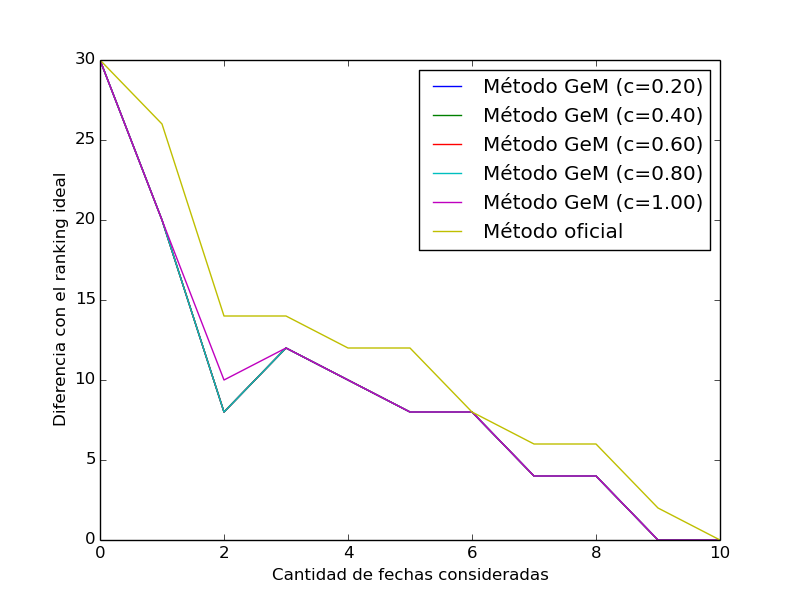
\includegraphics[width=.5\textwidth]{exp5_ejemplo_c_malo.png}
    }
    \subfloat[][Caso particular malo para GeM]{
        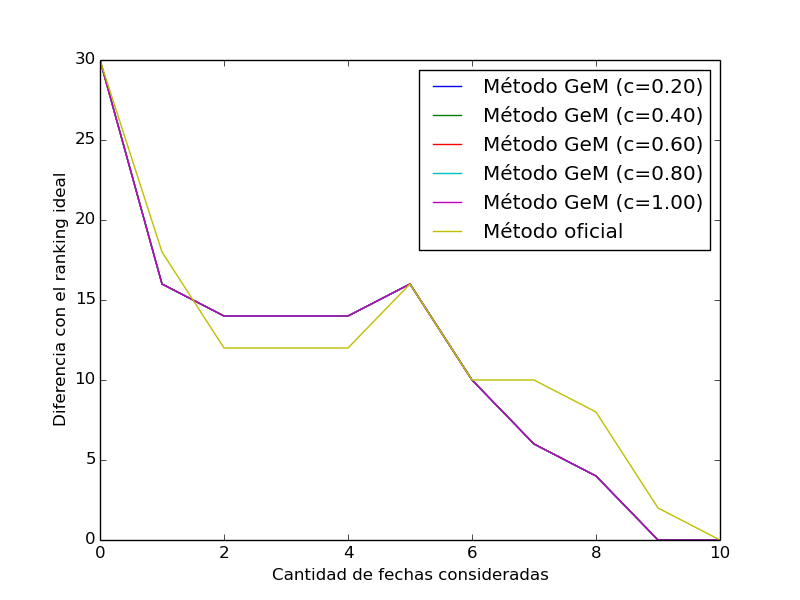
\includegraphics[width=.5\textwidth]{exp5_ejemplo_gem_malo.png}
        \label{subfig:exp5_gem_malo}
    }
    \caption{Casos Patol\'ogicos (10 equipos, $c = \alpha$)}
    \label{fig:exp5}
\end{figure}

\par Comparamos GeM con el orden oficial, establecido por asignación de puntos
(3-1-0) y confirmamos tambi\'en nuestra hip\'otesis de que en el caso promedio,
GeM se comporta mejor que el orden oficial de asignaci\'on de puntajes,
acerc\'andose más al ideal para cualquier cantidad de fechas.

\par Sin embargo tambi\'en encontramos semillas para las cuales esto no era real
en alg\'un punto (ver figura \ref{subfig:exp5_gem_malo}) por lo que tampoco
podemos generalizar esta conclusi\'on.

\par Por \'ultimo, dado que los dos casos ''patol\'ogicos'' fueron encontrados
con la instancia de pocos equipos (10) y no logramos encontrar una semilla que
los genere en el caso de muchos (50), podr\'iamos argumentar que GeM se comporta
''mejor'' cuando la cantidad de equipos es grande. Queda fuera de los alcances
de este trabajo confirmar m\'as sistem\'aticamente esa hip\'otesis, pero es un
buen trabajo futuro.
